\documentclass[11pt]{article}
    %	options include 12pt or 11pt or 10pt
    %	classes include article, report, book, letter, thesis
    
    \title{HW3}
    \author{Shane Drafahl}
    \date{13 September ,2017}
    \usepackage{graphicx}
    \usepackage{epstopdf}
    \usepackage{graphics}

    \begin{document}
    \maketitle

    1. Prove or disprove every finite language is recognized by some FA.
    $ \newline \newline $
    A finite language can be represented by a regular expression because
    if the language is finite then we can order the strings in some sort of order
    $ s_{0}, s_{1}, s_{2}, ..., s_{n} $ where n is equal to the number
    of strings substracted by 1 in the finite alphabet. We could simply union every string 
    together $ s_{0} + s_{1} + s_{2} + ... + s_{n} $ to make a regular expression. We know from
    2.7 of the LanguageBook.pdf from the Definition that a language L is regular iff
    it can be represented by a regular expression so we know a finite language is regular.
    The theorem states that a language is regular iff it is accepted by a finite automaton so 
    therefore we know that every finite language is recognized by some FA.
    $ \newline \newline $
    2. Define a DFA, simplified to the best of your abilities, that recognizes the language 
    L = $ \{\ w \in  { \{\ a,b \}\ }^{*} : $ w does not contain the substring abba $ \}\  $
    $ \newline \newline $
    \begin{figure1}
        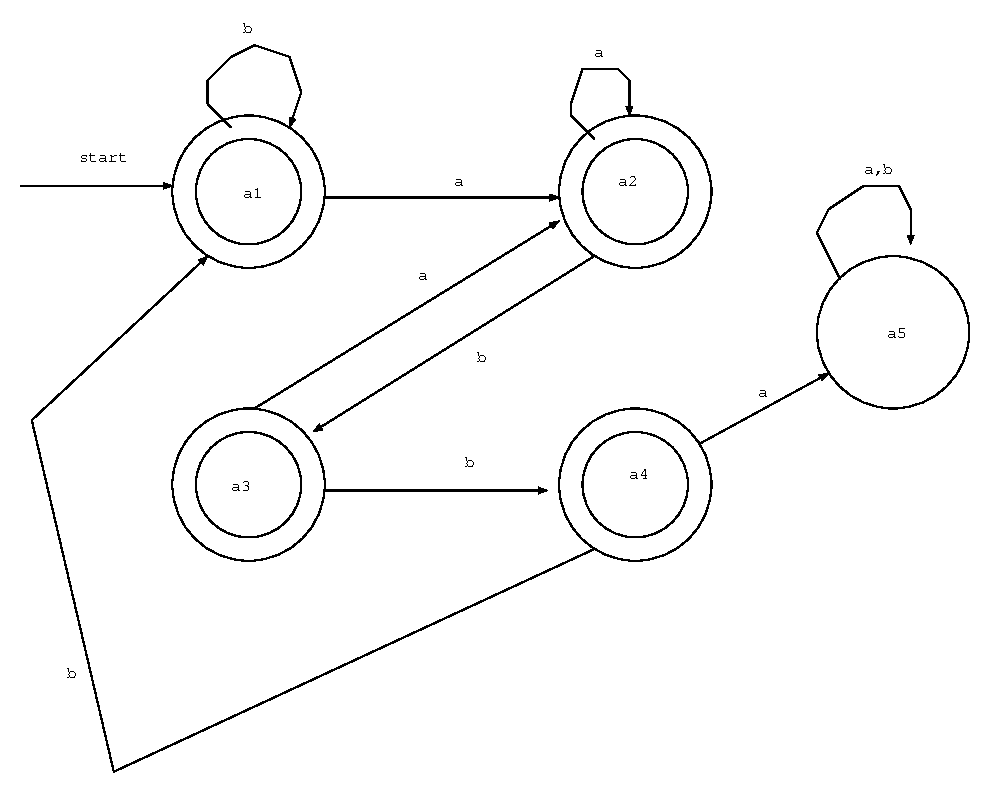
\includegraphics[scale=.7]{./hw3_1.eps}
    \end{figure1}
    $ \newline \newline $
    3. Define a DFA for the following language.
    $ \newline \newline $
    \begin{figure}
        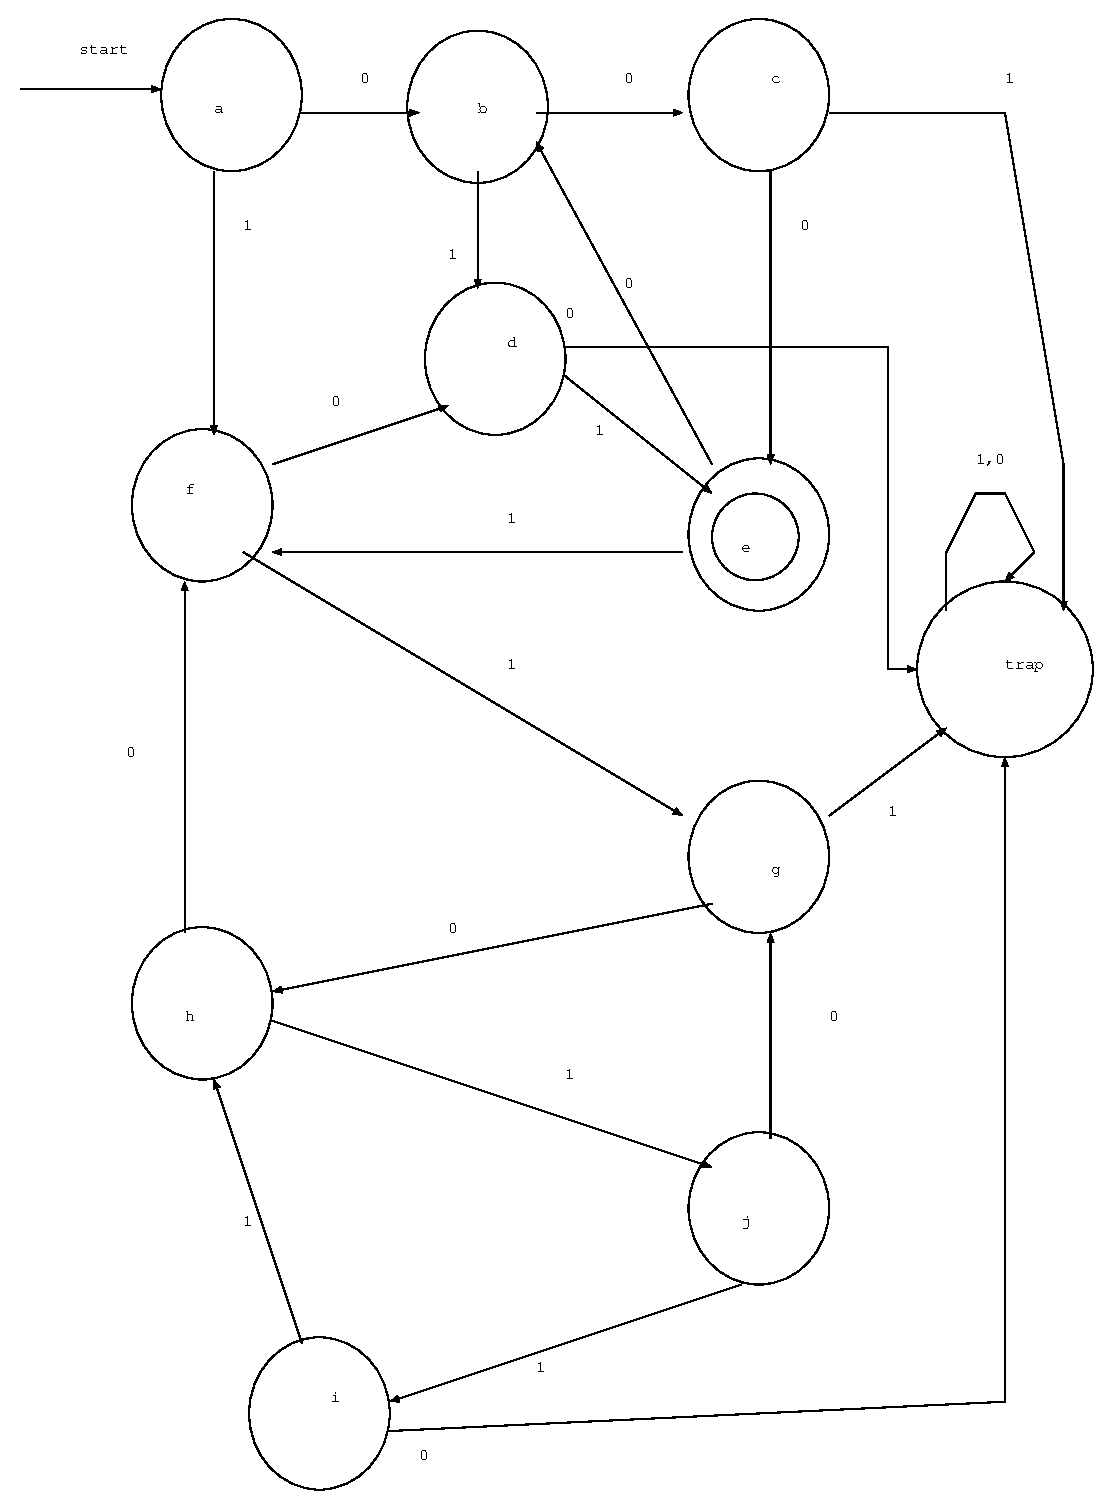
\includegraphics[scale=.7]{./hw3_2.eps}
    \end{figure}

    \end{document}